\documentclass[10pt,addpoints,answers]{exam}
% Entfernen Sie die Option answers, wenn Sie die Version für die Studenten ohne die Antwort-Hinweise kompilieren möchten
\usepackage[T1]{fontenc}
\usepackage[utf8]{inputenc}
\usepackage{amsmath}
\usepackage[left=1cm,right=1cm]{geometry}
\usepackage{graphicx}
\usepackage{float}
\usepackage{tikz}
\usetikzlibrary{positioning, calc}
\usepackage{amssymb}
\usepackage{amsfonts}
\usepackage{tikz}
\usetikzlibrary{patterns}
\usepackage{booktabs}


\begin{document}

\begin{center}
\textbf{\Huge Nachprüfung aus Quantitative Methoden 1 2025} \\
\vspace{0.5cm}
Jürgen Degenfellner\\
\vspace{0.5cm}
\textbf{\large 17.1.2025}
\end{center}
\vspace{1cm}

\noindent Name: \fbox{\begin{minipage}{0.4\linewidth}
        \vspace{1mm}
        \hspace{0.3\linewidth}
        \vspace{5mm}
    \end{minipage}} \\
    
\vspace{5mm} % Erhöhen Sie diesen Wert, um den Abstand zwischen den Boxen zu vergrössern

\noindent Matrikelnummer: \fbox{\begin{minipage}{0.4\linewidth}
        \vspace{1mm}
        \hspace{0.3\linewidth}
        \vspace{5mm}
    \end{minipage}}

\vspace{10mm}

\noindent In den folgenden Aufgaben sind immer \textbf{zwischen minimal null und maximal vier Antwortmöglichkeiten} korrekt. Die korrekten Antworten sind auf dem separaten Antwortblatt anzukreuzen. \textbf{Nur} die dort angekreuzten Antworten werden gewertet. \\
\\
Details Punktemodalitäten: Die minimale Punktezahl pro Frage ist 0, die maximale ist 4. Die Anzahl der Punkte pro Frage errechnet sich aus: Punktemaximum minus Anzahl der Fehler. Fehler sind \\
 - nicht angemalte Antworten, die jedoch richtig sind und \\
 - angemalte Antworten, die jedoch falsch sind. \\
\\
Folgende \textbf{Hilfsmittel} sind erlaubt: Ein A4 Blatt mit handschriftlichen Notizen, dokumentenechter Stift (kein Bleistift), schwarzer Filzstift für die Antworten, nicht-programmierbarer Taschenrechner. Notizblätter müssen gemeinsam mit der Prüfung abgegeben werden. 
\vspace{1cm}

Viel Erfolg!

\newpage

\begin{questions}

%1
\question Der Stichprobenkorrelationskoeffizient $r$ in Figure \ref{fig:korrelation} ist $-0.2486312$. 

\begin{figure}[H]
\centering
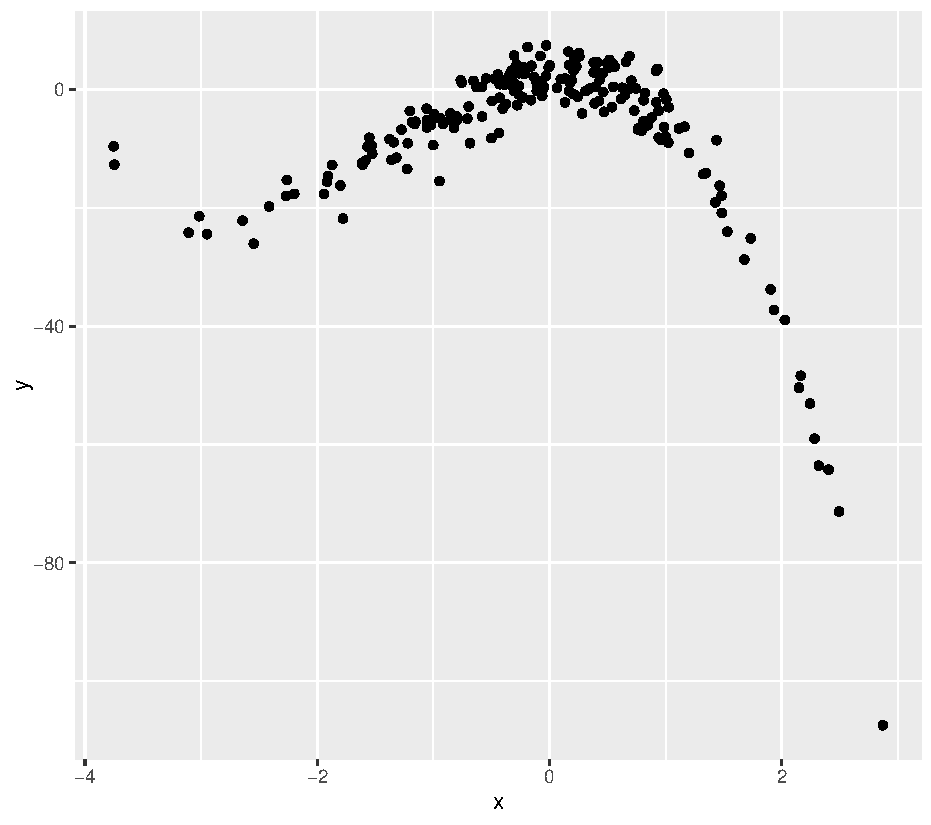
\includegraphics[width=0.6\linewidth]{./images/Frage_Korrelation.pdf}
\caption{Zusammenhang x,y}
\label{fig:korrelation}
\end{figure}

Welche Aussage(n) ist/sind korrekt?\\

\begin{choices}
\CorrectChoice Betrachtet man die Grafik, lässt sich der Zusammenhang gut durch eine Polynomfunktion 3. Grades beschreiben.
\CorrectChoice Sähe man nur die Daten ab $x=1$, wäre der Korrelationskoeffizient $r$ betragsmäßig höher.
\choice Die Korrelation ist ein geeignetes Maß, um diesen Zusammehang zu beschreiben.
\CorrectChoice Sähe man nur die Daten im Bereich von $x=-3$ bis $x=0$, wäre der Korrelationskoeffizient $r$ betragsmäßig höher.
\end{choices}

%2
\question Es soll die Unabhängigkeit der Variablen \textit{Bewegungstherapie} (Ja/Nein) 
und \textit{Schmerzlinderung} (Ja/Nein) untersucht werden. Die Teststatistik für 
den \(\chi^2\)-Test lautet:
\[
\chi^2 = \sum_{i,j} \frac{(X_{ij} - n \cdot \pi_{ij})^2}{n \cdot \pi_{ij}}
\]

\begin{center}
\begin{tabular}{|l|c|c|c|}
\hline
& Schmerzlinderung Ja & Schmerzlinderung Nein & Summe \\
\hline
Bewegungstherapie Ja & 35 & 10 & 45 \\
Bewegungstherapie Nein & 15 & 40 & 55 \\
\hline
Summe & 50 & 50 & 100 \\
\hline
\end{tabular}
\end{center}

Welche Aussage(n) ist/sind korrekt?\\

\begin{choices}
\CorrectChoice Wir dürfen annehmen, das Quantil der $\chi^2$-Verteilung bei der korrekten Anzahl von 
Freiheitsgraden und $\alpha=0.01$ ist $6.634897$. Dann ist $p$-Wert ist kleiner als $0.01$.
\choice $\mathbb{P}(\text{Schmerzlinderung} = "Ja") = 0.7777778$
\CorrectChoice Der Wert der Teststatistik ist $\chi^2 = 25.253$.
\choice Die Teststatistik hat $2$ Freiheitsgrade.
\end{choices}

%3
\question Welche Aussage(n) hinsichtlich des $p$-Wertes ist/sind korrekt?\\

\begin{choices}
\choice Der $p$-Wert ist die Wahrscheinlichkeit, dass die Nullhypothese wahr ist.
\choice Der $p$-Wert gibt die Wahrscheinlichkeit an, dass das Testergebnis falsch ist.
\choice Ein $p$-Wert grösser als 0.03 heisst, es gibt keinen Effekt (auf dem 3\% Niveau).
\CorrectChoice Der $p$-Wert gibt die Wahrscheinlichkeit an, unter der Annahme, dass die 
Nullhypothese wahr ist, den beobachteten Wert (der Teststatistik) oder einen "extremeren" (in Richtung $H_1$)
zu erhalten.
\end{choices}

%4
\question Wir betrachten zwei Ereignisse im Venn-Diagramm (Figure \ref{fig:venn_diagram}). 
Welche Aussage(n) ist/sind korrekt?

\begin{figure}[h!]
    \centering
    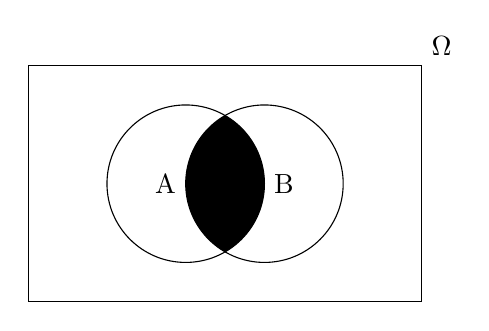
\begin{tikzpicture}
      % Das Rechteck für den gesamten Raum Omega
      \draw (0,0) rectangle (5,3) node[above right] {$\Omega$};
    
      % Zwei Kreise (A und B) mit schwarzem Schnittbereich
      \begin{scope}
        \clip (2,1.5) circle (1);
        \fill[black] (3,1.5) circle (1);
      \end{scope}
      \draw (2,1.5) circle (1) node[left] {A};
      \draw (3,1.5) circle (1) node[right] {B};
    \end{tikzpicture}
    \caption{Ereignisse \(A\) und \(B\) in \(\Omega\).}
    \label{fig:venn_diagram}
\end{figure}

\begin{choices}
\choice Da die Ereignisse nicht disjunkt (disjoint) sind, können sie auch nicht unabhängig (independent) sein.
\choice Die Wahrscheinlichkeit der Vereinigung $P(A \cup B)$ ist gleich groß oder größer als die Summe der 
Einzelwahrscheinlichkeiten $P(A) + P(B)$.
\choice $\mathbb{P}(A \cap B) = \emptyset$ (leere Menge).
\choice $\mathbb{P}(A \cap B) = \mathbb{P}(\Omega)$
\end{choices}

%5
\question Gegeben sei folgende Stichprobe: $ \mathbf{x} = (5.879049, 6.539645, 10.117417, 7.141017, 7.258575, 10.430130, 7.921832)$\\
\\
Welche Aussage(n) ist/sind korrekt?\\

\begin{choices}
\CorrectChoice Die Spannweite beträgt $4.551081$. 
\CorrectChoice Der Median ist $7.258575$. 
\CorrectChoice Die Stichprobenstandardabweichung beträgt $1.743619$.
\CorrectChoice $6.539645$ und $7.258575$ sind Modi dieser Stichprobe.
\end{choices}

%6
\question Wir erzeugen mit R eine Stichprobe vom Umfang $n=100$ ($x_1, \dots, x_{100}$) einer normalverteilten 
Zufallsvariable mit $\mathbb{E}(X) = \mu = 10$ und $\sigma = 10$. Mit $\widehat{\mathbb{V}ar}(.)$ ist die 
aus der Stichprobe geschätze Varianz gemeint.\\
\\
Welche Aussage(n) ist/sind korrekt?\\

\begin{choices}
\choice $\mathbb{E}(\frac{X - \mu}{\sigma}) = 1$.
\choice Der Mittelwert von $z_i = \frac{x_i - \bar{x}}{s}$ ist ungefähr $1$.
\CorrectChoice $\mathbb{V}ar(\frac{X - \mu}{\sigma}) = 1$.
\CorrectChoice $\widehat{\mathbb{V}ar}(\frac{x_i - \bar{x}}{s}) = 1$.
\end{choices}

%7
\question Welche Aussage(n) in Bezug auf Figure \ref{fig:x_density} ist/sind wahr?

\begin{figure}[H]
    \centering
    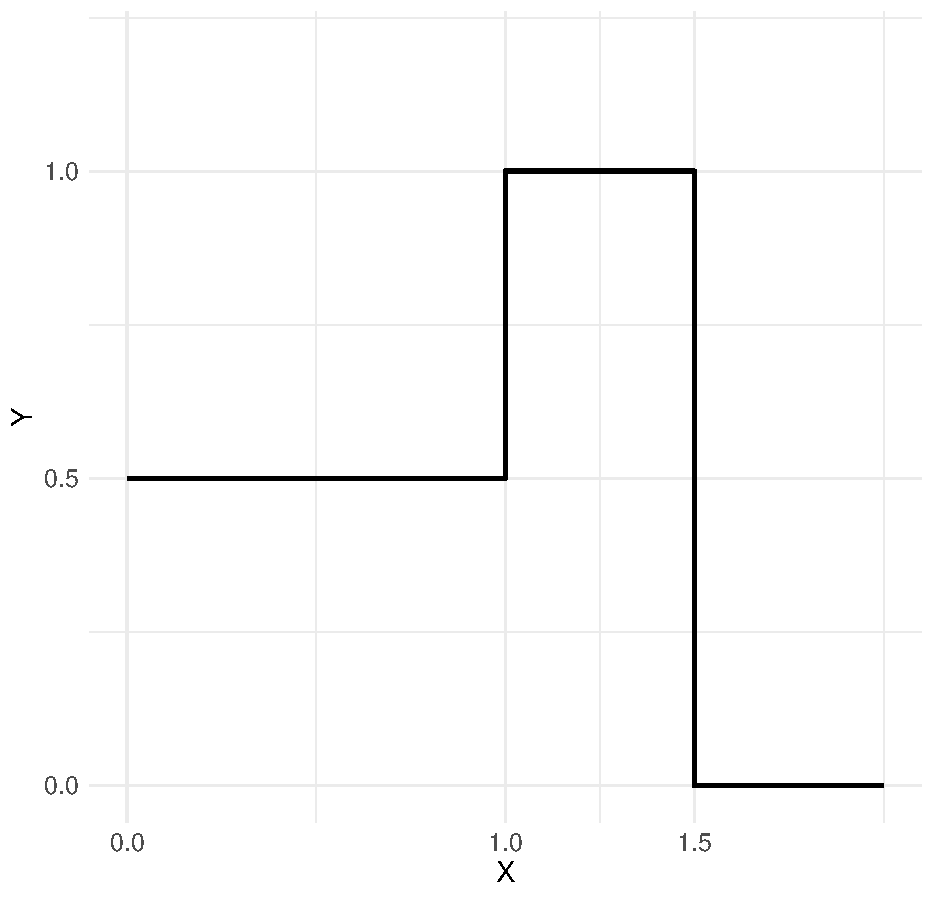
\includegraphics[width=0.3\linewidth]{./images/x_density_rectangle.pdf}
    \caption{Dichteplot für $X$?}
    \label{fig:x_density}
\end{figure}

\begin{choices}
\choice $\mathbb{P}(X > 1.5) = 1$.
\CorrectChoice Es handelt sich um eine Wahrscheinlichkeitsdichte für die Zufallsvariable $X$.
\CorrectChoice $\mathbb{P}(X \in [0,0.5]) = 0.25$. 
\CorrectChoice Man kann den Erwartungswert dieser Verteilung auch ohne Integral berechnen: 
Die Wahrscheinlichkeit, dass $X$ in $[0,1]$ liegt, wird $X=0.5$ zugeordnet. 
Die Wahrscheinlichkeit, dass $X$ in $[1,1.5]$ liegt, wird $X=1.25$ zugeordnet.
Wenn man nun den Erwartungswert dieser diskreten Zufallsvariable berechnet, erhält man $0.875$.
\end{choices}

%8
\question Welche der folgenden Aussage(n) über untige Tabelle ist/sind korrekt?

\[
\begin{array}{|c|c|}
\hline
y & P(Y = y) \\
\hline
a & 0.1 \\
b & 0.4 \\
rot & 0.2 \\
blau & 0.2 \\
Steuermann & 0.1 \\
\hline
\end{array}
\]

\begin{choices}
\choice $Y$ ist eine ordinale (geordnete) Zufallsvariable.
\CorrectChoice $\mathbb{P}(Y \text{ ist eine Farbe}) = 0.4$.
\choice $\mathbb{P}(Y \le b) = 0.5$.
\choice $\mathbb{P}(Y = "ab") = 0.5$.
\end{choices}

%9
\question Ein medizinischer Test wird verwendet, um eine bestimmte Krankheit zu erkennen. 
Der Test hat folgende Eigenschaften:\\
- Sensitivität: 92\%\\
- Spezifität: 97\%\\
- Die Prävalenz der Krankheit in der Bevölkerung beträgt 1\%.\\

Welche Aussage(n) ist/sind korrekt?\\

\begin{choices}
\CorrectChoice Die Wahrscheinlichkeit, dass der Test positiv ist, wenn die Person die Krankheit nicht hat, beträgt 3\%.
\choice Die Wahrscheinlichkeit, dass die Person die Krankheit hat, wenn der Test positiv ist, beträgt 27,65039\%.
\CorrectChoice Die Wahrscheinlichkeit, dass der Test positiv ist, wenn die Person die Krankheit hat, beträgt 92\%.
\choice Die Wahrscheinlichkeit für einen positiven Test ist 5,46\%.
\end{choices}

%10
\question Wir erinnern uns and die Ausführungen aus dem R-File \textit{H\_0\_and\_the\_truth.R} (siehe Figure \ref{fig:screenshot_H0_and_truth}). Welche Aussage(n) ist/sind hinsichtlich Hypothesentesten korrekt?

\begin{figure}[H]
\centering
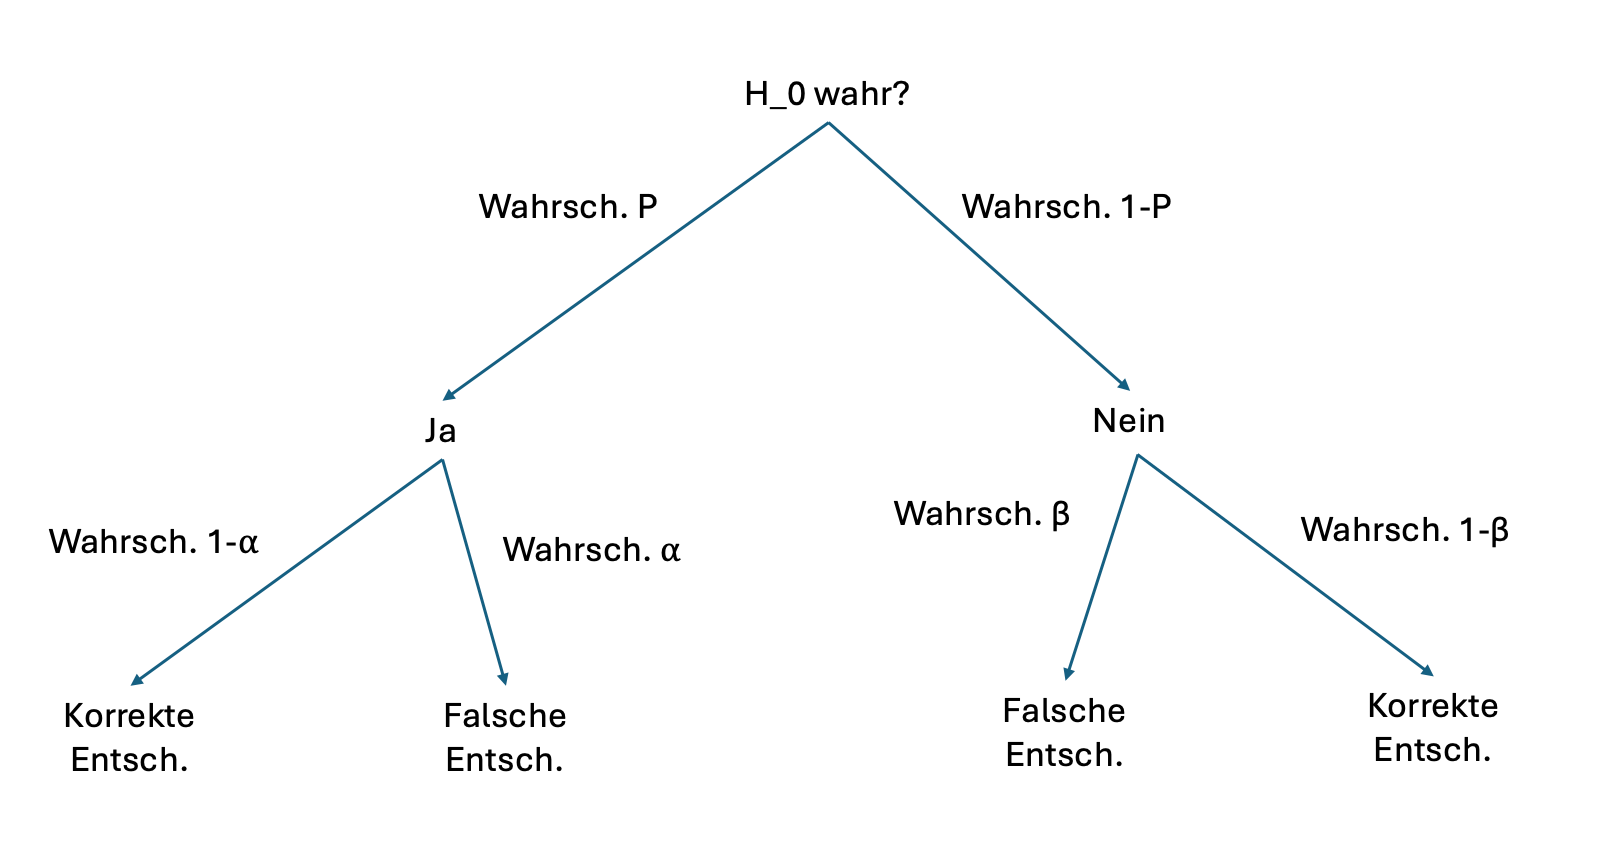
\includegraphics[width=0.6\linewidth]{./images/h_0_and_truth_new.png}
\caption{$H_0$ and the truth}
\label{fig:screenshot_H0_and_truth}
\end{figure}

\begin{choices}
\CorrectChoice Falls $\alpha=0.05$, $\beta=0.2$ und $P=0.5$, dann ist die Wahrscheinlichkeit dafür eine falsche Testentscheidung zu treffen $12.5\%$.
\CorrectChoice Ein $\beta$-Fehler oder \textit{Fehler 2. Art} ist die Wahrscheinlichkeit, unter der Annahme, dass $H_0$ falsch ist, $H_0$ fälschlicherweise nicht abzulehnen. 
\CorrectChoice Ein $\alpha$-Fehler oder \textit{Fehler 1. Art}, ist die Wahrscheinlichkeit, unter der Annahme, dass $H_0$ wahr ist, diese fälschlicherweise abzulehnen.
\CorrectChoice $1-\beta$ heißt auch \textit{Power}.
\end{choices}

%11
\question Wir betrachten den QQ-Plot (gegen die theoretischen Quantile der Normalverteilung) und das Histogramm einer Stichprobe $x_1, \dots , x_{100}$ vom Umfang $100$ (siehe Figure \ref{fig:qqplot_density}). 
Die rote Dichtekurve rechts ist die Dichte einer Normalverteilung mit $\mu = \bar{x}$ und $\sigma = s$.\\
\\
Welche Aussage(n) ist/sind  korrekt?

\begin{figure}[H]
    \centering
    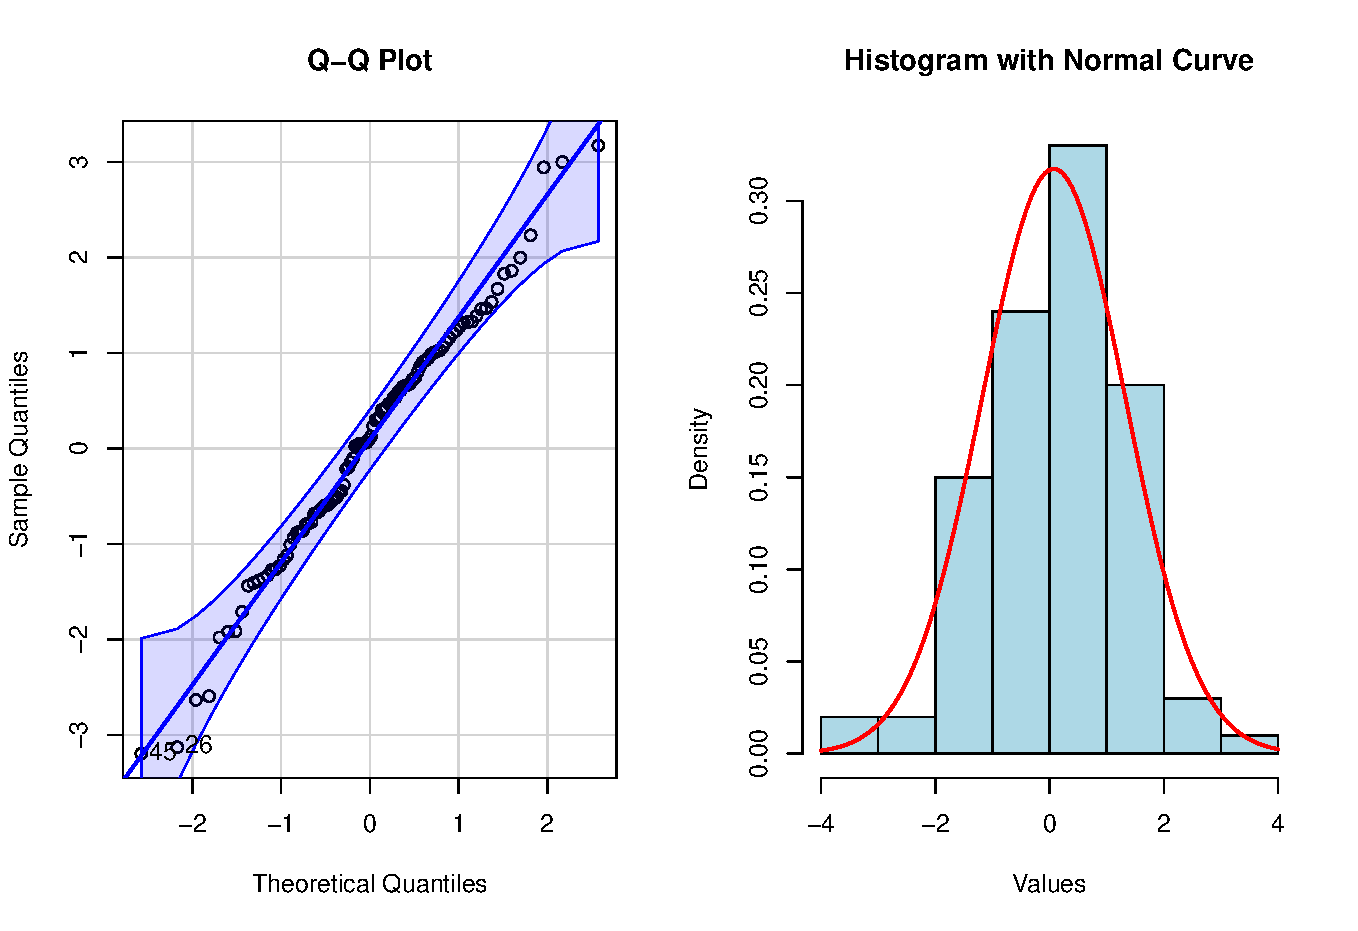
\includegraphics[width=0.8\linewidth]{./images/t_verteilung_normal_fragezeichen.pdf}
    \caption{QQ-Plot und Histogramm mit Dichtekurve einer Normalverteilung}
    \label{fig:qqplot_density}
    \end{figure}

\begin{choices}
\choice Normalverteilung kann ausgeschlossen werden.
\choice Der Shapiro-Wilk-Test zeigt einen $p$-Wert von $0.5761$. Wir können daher schließen, dass die Stichprobe aus einer Normalverteilung stammt.
\CorrectChoice Der QQ-Plot ist mit einer Normalverteilung vereinbar.
\CorrectChoice Der QQ-Plot könnte auch von einer $t$-Verteilung mit höherer Anzahl an Freiheitsgraden stammen.
\end{choices}

%12
\question Wir führen einen Bayes $t$-Test durch, um die Gleichheit der Mittelwerte zweier Gruppen zu testen (siehe Figure \ref{fig:bayes_t_test}).\\
\\
Welche Aussage(n) ist/sind korrekt?

\begin{figure}[H]
\centering
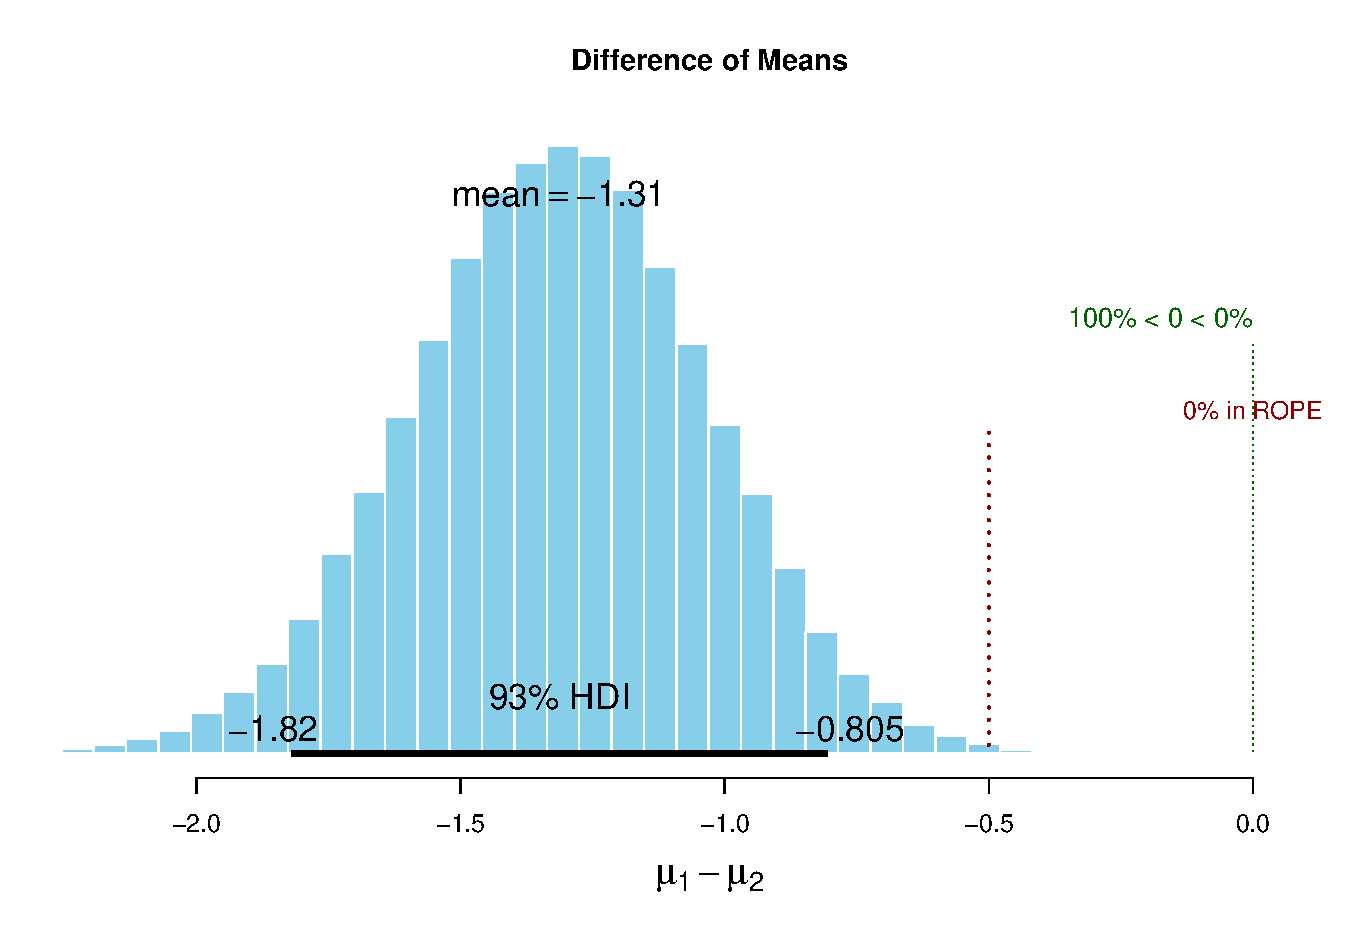
\includegraphics[width=0.8\linewidth]{./images/Bayes_t_Test.pdf}
\caption{Bayes $t$-Test}
\label{fig:bayes_t_test}
\end{figure}

\begin{choices}
\choice Die Wahrscheinlichkeit, dass die Mittelwertdifferenz kleiner als $0$ ist, beträgt $0.93$.
\choice Wir schließen: $\mu_1 > \mu_2$.
\choice Mit 95\%iger Wahrscheinlichkeit liegt die Mittelwertdifferenz zwischen $-1.82$ und $-0.805$.
\CorrectChoice Die Testentscheidung lautet: Die Mittelwertdifferenz ist wahrscheinlich kleiner als $0$.
\end{choices}

%13
\question Wir führen ein Zufallsexperiment aus und definieren zwei Ereignisse $A$ und $B$.
Die Wahrscheinlichkeit, dass $A$ eintritt, ist $0.3$. Die Wahrscheinlichkeit, dass $B$ eintritt, ist
$0.15$. Die Wahrscheinlichkeit, dass $A$ und $B$ gleichzeitig eintreten, ist $0.07$.\\
\\
Welche Aussage(n) ist/sind korrekt?

\begin{choices}
\choice $A$ und $B$ sind disjunkt.
\choice $\mathbb{P}(A \cup B) = 0.34$
\choice Wäre Ereignis $B$ unmöglich, wäre $\mathbb{P}(A \cup B) = 0$
\choice $A$ und $B$ sind unabhängig.
\end{choices}

%14
\question Unter der Nullhypothese "Student rät bei allen Antworten", ist die Anzahl der korrekten Antworten $X$
beim Test, den wir gerade schreiben, binomialverteilt: $X \sim Binomial(n=100, p=0.5)$.
Tabelle \ref{tab:binomialwerte} zeigt einige Werte der
Verteilungsfunktion und Masse dieser Binomialverteilung. 
Wir führen einen zweiseitigen Hypothesentest durch und legen fest: $\alpha = 0.04$.\\
Eine Kollegin von dir erreicht bei diesem Test $x=30$ korrekte Antworten.
\\
\begin{table}[h!]
    \centering
    \caption{Einige Werte der Verteilungsfunktion und Masse der Binomialverteilung}
    \label{tab:binomialwerte}
    \begin{tabular}{|c|c|c|}
    \hline
    $x$ & $F(x)$ & $p(x)$ \\
    \hline
    10  & 0.000 & 0.000 \\
    20  & 0.000 & 0.000 \\
    30  & 0.000 & 0.000 \\
    40  & 0.028 & 0.011 \\
    50  & 0.540 & 0.080 \\
    60  & 0.982 & 0.011 \\
    70  & 1.000 & 0.000 \\
    80  & 1.000 & 0.000 \\
    90  & 1.000 & 0.000 \\
    100 & 1.000 & 0.000 \\
    \hline
    \end{tabular}
    \end{table}

Welche Aussage(n) ist/sind korrekt?
\\
\begin{choices}
\CorrectChoice Der $p$-Wert für diesen zweiseitigen Test beträgt (laut Tabelle) ca. $0.000$.
\CorrectChoice Der Erwartungswert dieser Binomialverteilung ist $50$.
\choice Wir schließen, dass die Kollegin geraten hat.
\choice $\mathbb{P}(X \in [50, 60]) = 0.091$.
\end{choices}

%15
\question Welche Aussage(n) ist/sind hinsichtlich Erwartungswert und Varianz einer Zufallsvariable korrekt?
\\
\begin{choices}
\CorrectChoice Eine Zufallsvariable $X$ hat Varianz $2$. Die Zufallsvariable $Y = 2X$ hat Varianz $8$.
\CorrectChoice Varianz ist die erwartete quadratische Abweichung vom Erwartungswert $\mathbb{E}(X)$.
\CorrectChoice Der Erwartungswert ist der Massenschwerpunkt über der Dichtekurve einer (stetigen) Zufallsvariable.
\CorrectChoice Für eine diskrete Zufallsvariable $X$ ist der Erwartungswert die mit den 
Eintrittswahrscheinlichkeiten $\mathbb{P}(X = x_i)$ gewichtete Summe der möglichen Werte von $X$.
\end{choices}

%16
\question Welche Aussage(n) über das Bayes-Theorem $p(\theta | x) = \frac{p(x | \theta) \cdot p(\theta)}{p(x)}$ ist/sind korrekt?
\\
\begin{choices}
\choice $p(x)$ stellt das Vorwissen dar, das man über den interessierenden Parameter $\theta$ hat.
\choice $p(x | \theta)$ nennt man auch \textit{posterior distribution} des interessierenden Parameters $\theta$.
\CorrectChoice $p(x)$ ist im Allgemeinen schwer zu berechnen, weshalb man Monte Carlo Methoden verwendet.
\CorrectChoice In der Bayes-Praxis erspart man sich die Bestimmung der Verteilung einer Teststatistik unter $H_0$.
\end{choices}

%17
\question Welche Aussage(n) hinsichtlich Figure \ref{fig:side_by_side} ist/sind korrekt?\\

\begin{figure}[h!]
    \centering
    % First Image
    \begin{minipage}{0.45\textwidth}
        \centering
        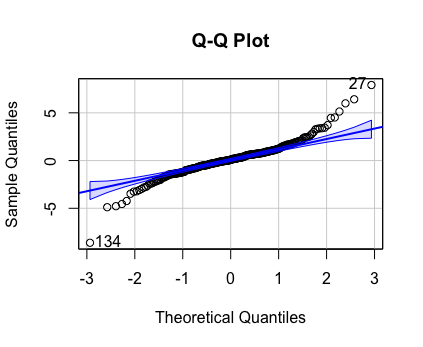
\includegraphics[width=\linewidth]{./images/one_sample_t_test_qqplot_Dez_24.png}
    \end{minipage}
    \hfill
    % Second Image
    \begin{minipage}{0.45\textwidth}
        \centering
        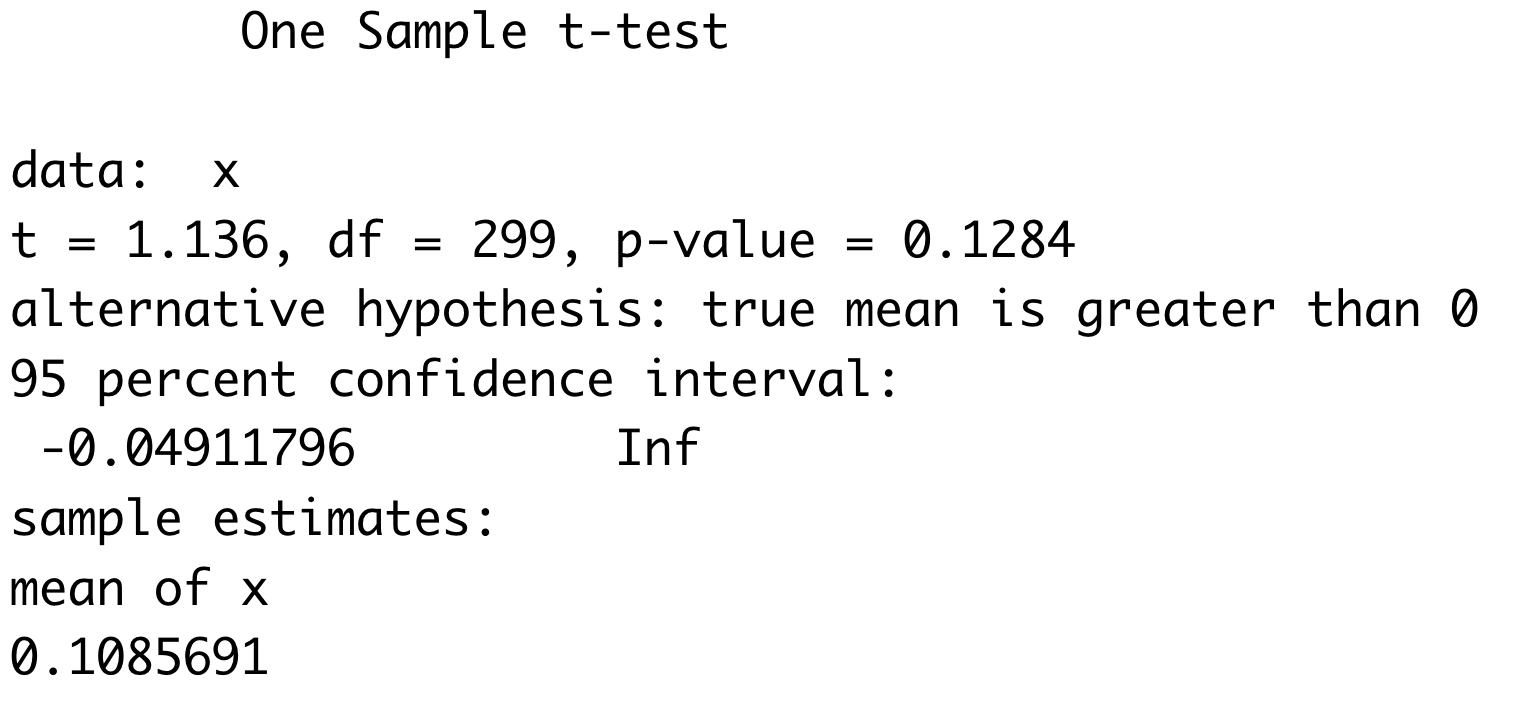
\includegraphics[width=\linewidth]{./images/one_sample_t_test_Dez_24.png}
    \end{minipage}
    \caption{QQ-Plot der Daten (gegen Normalverteilung) und R-Output des $t$-Tests.}
    \label{fig:side_by_side}
\end{figure}

\begin{choices}
\choice Da das QQ-Plot darauf hinweist, dass die Daten nicht normalverteilt sind, kann der $t$-Test nicht angewendet werden.
\choice Es wurde ein zweiseitiger Hypothesentest durchgeführt.
\CorrectChoice Die Stichprobengröße ist $n = 300$.
\choice $\bar{x} = 1.136$
\end{choices}

%18
\question Welche Aussage(n) hinsichtlich \textit{Confidence Intervals} (frequentistische Statistik) und \textit{Credible Intervals} (Bayes) ist/sind korrekt?
\\
\begin{choices}
\CorrectChoice Für ein konkretes (klassisches) Konfidenzinterval gilt: Der wahre aber unbekannte Parameter ist darin enthalten oder nicht.
\choice Sei $[a,b]$ ein 95\%-Konfidenzintervall für einen unbekannten aber, festen Parameter. Die Wahrscheinlichkeit, dass der unbekannte aber wahre Parameter in diesem Intervall liegt, ist 95\%.
\CorrectChoice Sei $[a,b]$ ein 95\% \textit{Credible interval}, das wir z.B. durch einen Bayes-$t$-Test gefunden haben. Die Wahrscheinlichkeit, dass der unbekannte Parameter im Interval liegt, ist 95\%.
\CorrectChoice Wenn man viele (klassische 95\%) Konfidenzintervalle erzeugt, überdecken ca. 95\% der Intervalle den wahren, aber unbekannten Parameter.
\end{choices}

%19 cortest
\question Leider gingen beim Screenshot der Wert der $t$-Statistik und der $p$-Wert verloren. 
Zum Glück sind wir Experten.
Welche Aussage(n) hinsichtlich Figure \ref{fig:cortest} ist/sind korrekt?
 \\
 \begin{figure}[h!]
    \centering
    % First Image
    \begin{minipage}{0.7\textwidth}
        \centering
        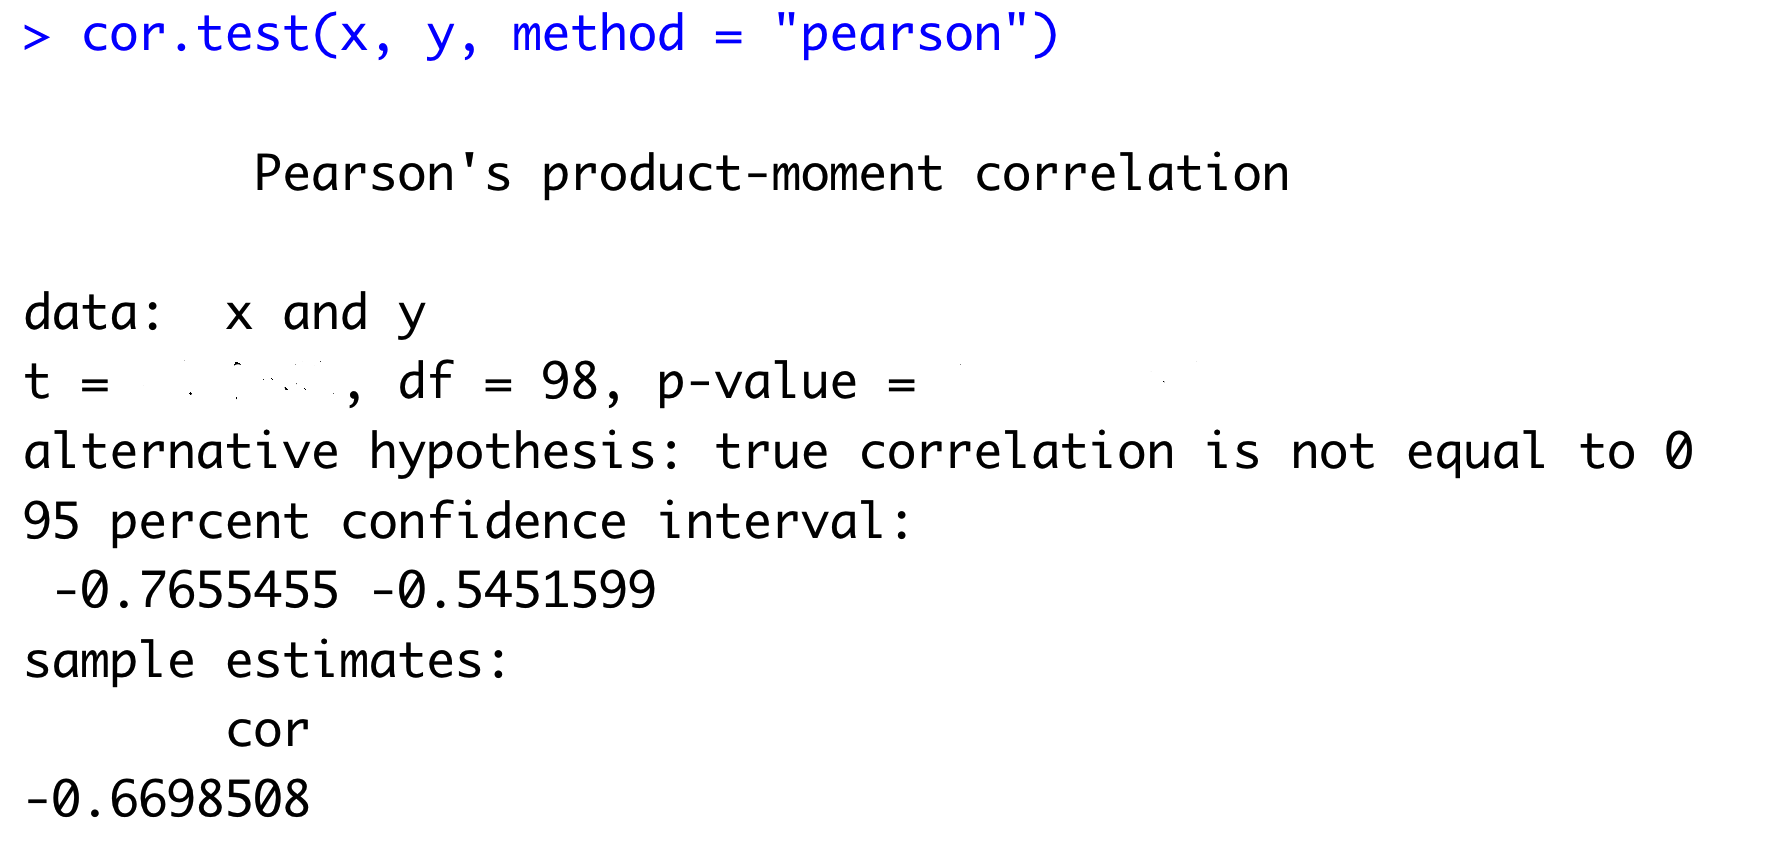
\includegraphics[width=\linewidth]{./images/cortest_output_r.png}
    \end{minipage}
    \hfill
    % Second Image
    \begin{minipage}{0.7\textwidth}
        \centering
        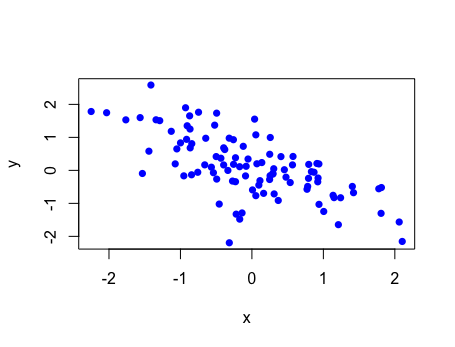
\includegraphics[width=\linewidth]{./images/cortest_scatterplot.png}
    \end{minipage}
    \caption{R-Output und Scatterplot.}
    \label{fig:cortest}
\end{figure}

\begin{choices}
\choice Man kann aufgrund des R-Outputs nicht sagen, ob der $p$-Wert kleiner als $0.05$ ist.
\choice Der Scatterplot deutet an, dass die Daten nicht durch einen linearen Trend beschrieben werden können.
\choice Der wahre aber unbekannte Parameter ($\rho$) liegt mit 95\%iger Wahrscheinlichkeit im angegebenen Konfidenzintervall.
\choice $H_0: \rho \ge 0$.
\end{choices}


%20
\question In Figure \ref{fig:bimodal_prior} ist eine Prior Verteilung für den Therapieeffekt
$\theta$ einer umstrittenen neuen Therapie zu sehen.\\
Welche Aussage(n) ist/sind korrekt?
\\
\begin{figure}[H]
    \centering
    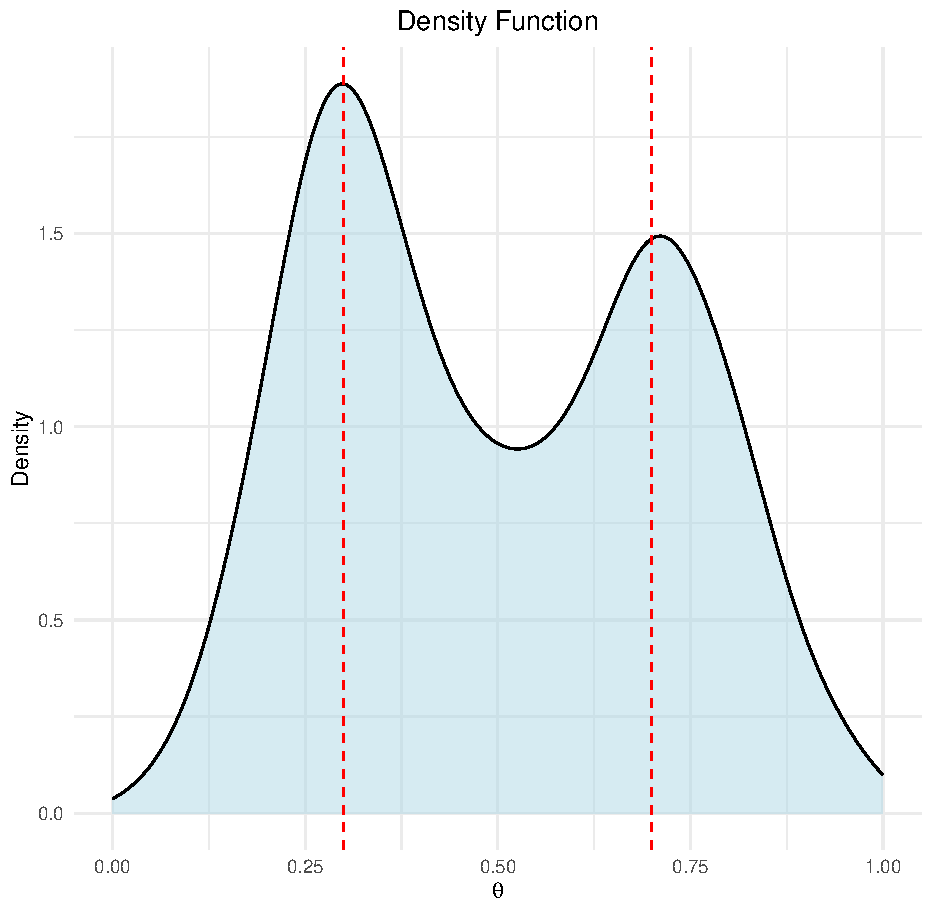
\includegraphics[width=0.6\linewidth]{./images/bimodal_prior.pdf}
    \caption{A priori Dichte des Therapieeffekts}
    \label{fig:bimodal_prior}
\end{figure}

\begin{choices}
\CorrectChoice Man ist sich a priori nicht ganz sicher, wie oft die Therapie wirkt. 
Es wurden hohe und niedrige Werte beobachtet und daher könnte man diese Art von Prior wählen.
\CorrectChoice Werte um $\theta = 0.3$ und $\theta=0.7$ hält man a priori für wahrscheinlicher als Werte um $\theta=0.5$.
\CorrectChoice Würde man in einer neuen Studie einen Therapieeffekt von $\theta=0.92$ beobachten, 
würde die a posteriori Verteilung rechts höher werden (verglichen mit der Prior).
\CorrectChoice Die a priori Verteilung ist zwar bimodal, 
Therapieeffekte um $\theta=0.5$ sind aber keinesfalls ausgeschlossen (a priori).
\end{choices}

%21
\question Angenommen, wir wissen, dass die Varianzen in beiden Gruppen gleich sind. 
Welche Aussage(n) ist/sind hinsichtlich Figure \ref{fig:two_sample_t_test} korrekt?
\\
\begin{figure}[H]
    \centering
    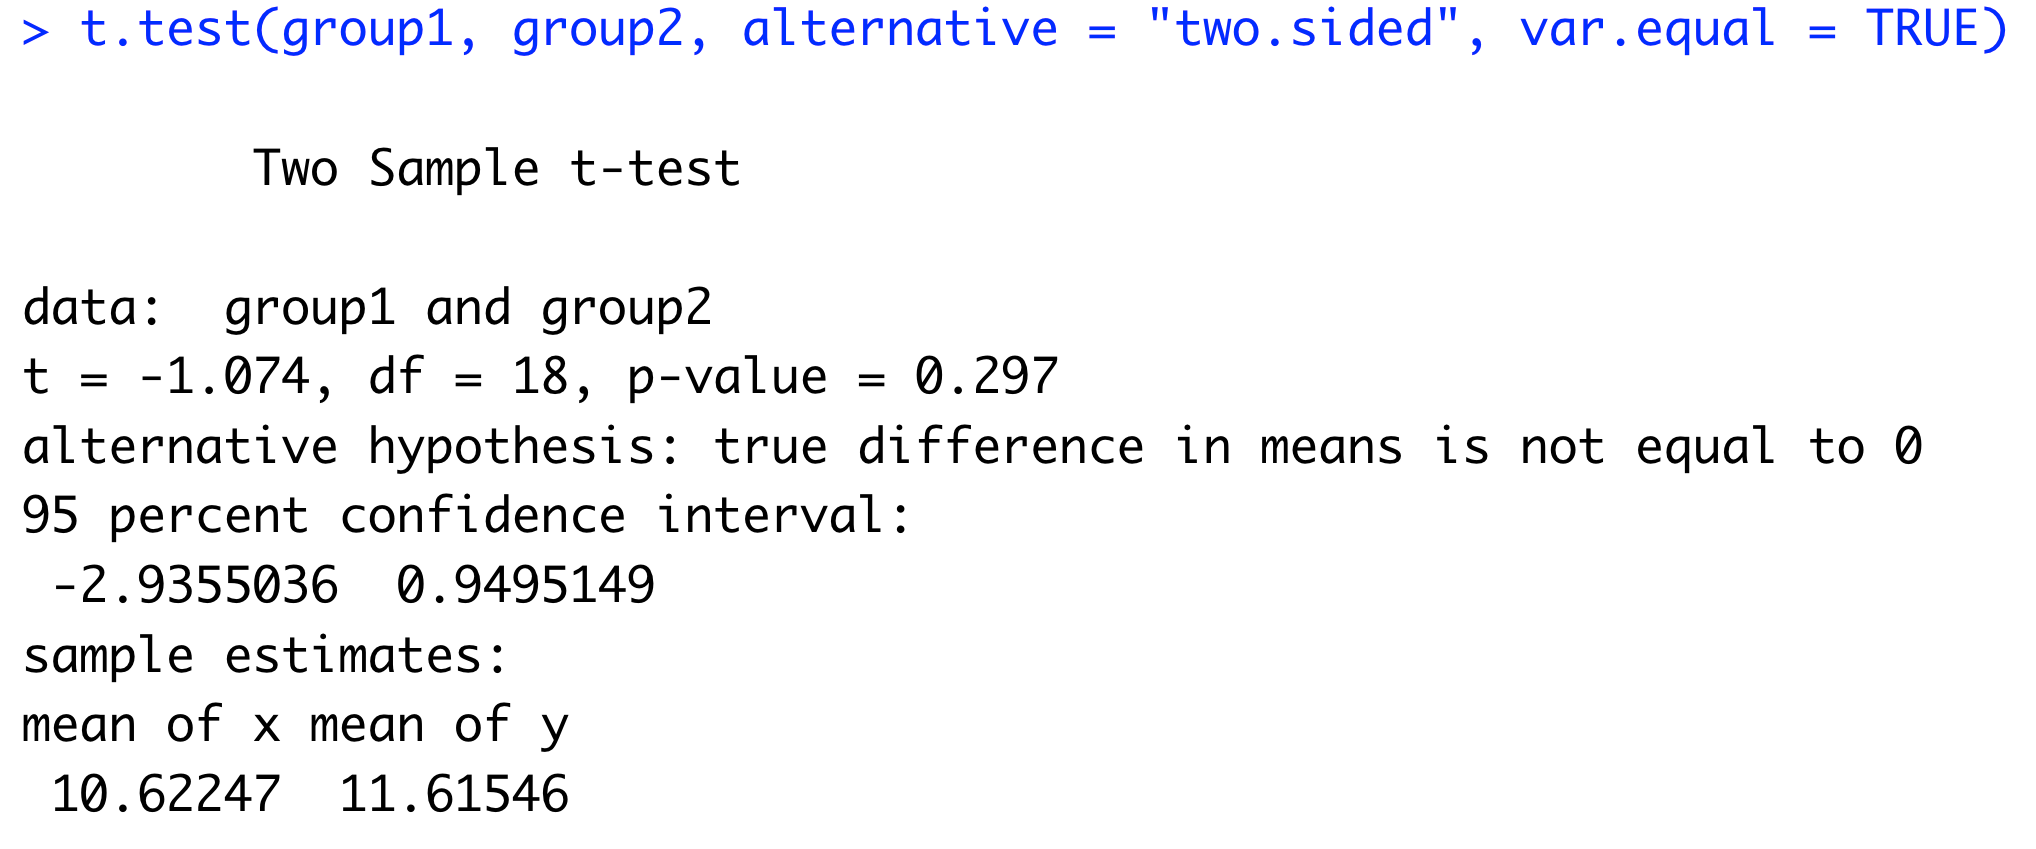
\includegraphics[width=0.6\linewidth]{./images/two_sample_t_test.png}
    \caption{R output}
    \label{fig:two_sample_t_test}
\end{figure}

\begin{choices}
\choice Die sample size $n=19$.
\choice Hier bekommt man kein "signifikantes" Ergebnis. 
Daraus folgt, dass es keinen Gruppenunterschied gibt.
\choice Angenommen, es gäbe einen Gruppenmittelunterschied. 
Mit höherer Stichprobengröße würde man die gleiche Schlussfolgerung tätigen.
\choice $\bar{x} - \bar{y} > 0$.
\end{choices}

%22
\question Welche Aussage(n) ist/sind hinsichtliche Bayes Statistik korrekt?
\\
\begin{choices}
\CorrectChoice Die Posterior Verteilung ist ein Kompromiss zwischen Prior und der Likelihood (den Daten).
\CorrectChoice Bei starkem Vorwissen (gute Studienlage) müssen viele Daten vorliegen, um die Prior Verteilung maßgeblich zu verändern.
\CorrectChoice Die Reihenfolge der Daten spielt bei der Bayes-Statistik keine Rolle (Bayes Updating).
\CorrectChoice Im Gegensatz zur frequentistischen Statistik, bekommt man bei der Bayes-Statistik eine Wahrscheinlichkeitsverteilung für den interessierenden Parameter.  
\end{choices}

%23
\question Welche Aussage(n) über den Zentralen Grenzverteilungssatz ist/sind korrekt?\\

\begin{choices}
\CorrectChoice Wenn die \(X_i\) Gamma-verteilt sind (und die restlichen Voraussetzungen für das Theorem zutreffen), so ist \(\bar{X}\) approximativ normalverteilt bei großem \(n\).
\CorrectChoice Wenn die \(X_i\) Binomial-verteilt sind (und die restlichen Voraussetzungen für das Theorem zutreffen), so ist \(\bar{X}\) approximativ normalverteilt bei großem \(n\).
\choice Die Verteilung von \(\frac{\bar{X} - \mu}{\sigma / \sqrt{n}}\) hängt von der Verteilung der \(X_i\) ab ($n$ gross).
\CorrectChoice \(\mathbb{V}ar(\bar{X}) = \frac{\sigma^2}{n}\) ($n$ gross).
\end{choices}

%24
\question Wir machen eine kleine Umfrage und fragen $130$ Studenten im Master, 
ob sie Mathe-Freaks sind und erhalten dabei folgende (fiktive) Zahlen (siehe Figure \ref{fig:mathefreaks}).
Welche Aussage(n) ist/sind korrekt?
\\
\begin{figure}[h!]
    \centering
    % First Image
    \begin{minipage}{0.7\textwidth}
        \centering
        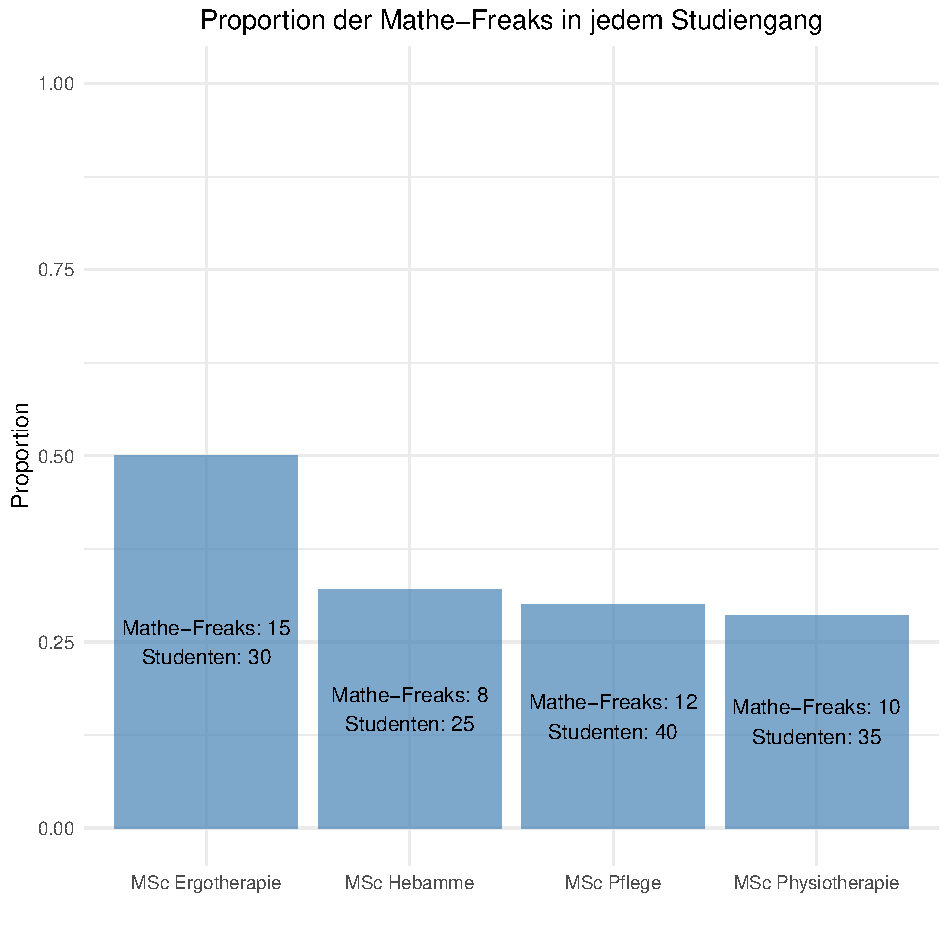
\includegraphics[width=\linewidth]{./images/mathe_freak_proportions.pdf}
    \end{minipage}
    \hfill
    % Second Image
    \begin{minipage}{0.7\textwidth}
        \centering
        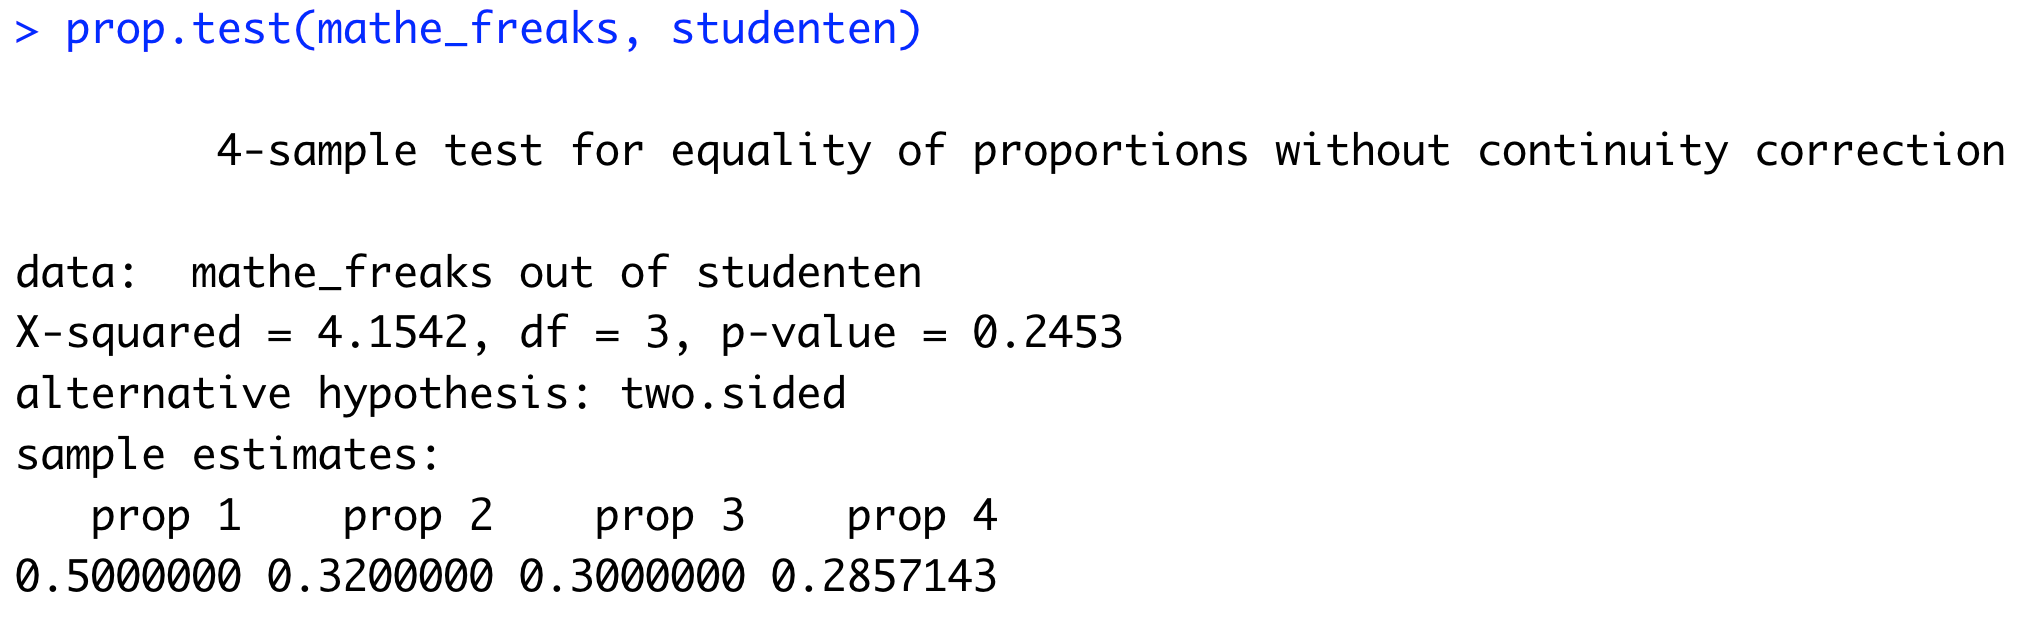
\includegraphics[width=\linewidth]{./images/mathe_freaks_R.png}
    \end{minipage}
    \caption{Barplot und R-Output.}
    \label{fig:mathefreaks}

\end{figure}
\begin{choices}
\choice Es handelt sich um einen einseitigen Test, da die $\chi^2$-Verteilung der Teststatistik nur nicht-negative Werte annimmt.
\CorrectChoice Die beobachteten Unterschiede in den Proportionen sind durch Zufall alleine gut erklärbar. 
\CorrectChoice Drei Freiheitsgrade hat man, da man bei bekannten Randsummen lediglich 3 
Zahlen in der $4$ mal $2$ Tabelle wissen muss, um diese vollständig zu kennen.
\CorrectChoice Den $p$-Wert könnte man sich direkt in R mit der Verteilungsfunktion der 
$\chi^2$-Verteilung mit drei Freiheitsgraden berechnen.
\end{choices}

%25
\question Welche der folgenden Aussage(n) über (einfache nicht-parametrische) Bootstrap Konfidenzintervalle ist/sind korrekt?\\

\begin{choices}
\choice Bootstrap-Konfidenzintervalle basieren auf der $t$-Verteilung und benötigen Normalverteilungsannahmen.
\choice Die Breite eines Bootstrap-Konfidenzintervalls hängt nicht von der (originalen) Stichprobengröße ab.
\CorrectChoice Bootstrap-Konfidenzintervalle werden durch wiederholtes Ziehen von Stichproben mit Zurücklegen aus den Originaldaten erstellt.
\choice Das Bootstrap-Verfahren liefert exakte Konfidenzintervalle unabhängig von der Verteilung der Daten.
\end{choices}



\printanswers
\end{questions}



\end{document}
